\documentclass{beamer}
\usetheme{Berkeley}
% \usetheme{Boadilla}
%\usetheme{Madrid}
%\usetheme{Montpellier}
%\usetheme{Warsaw}
%\usetheme{Copenhagen}
%\usetheme{Goettingen}
%\usetheme{Hannover}
%\usetheme{PaloAlto}
%\usetheme{AnnArbor}
%\usetheme{Bergen}

%\usepackage{beamerthemesplit}


\usepackage{amscd,amsxtra,amsthm}
%\usepackage[all]{xy}
%\usepackage{etex}
%\usepackage{pictex}
\usepackage{graphicx}
\usepackage{mathtools}

\theoremstyle{conjecture1}
%\newtheorem{conjecture}[theorem]{Conjecture}
\newtheorem{conjecture1}[theorem]{Conjecture 1}
\theoremstyle{conjecture2}
%\newtheorem{conjecture}[theorem]{Conjecture}
\newtheorem{conjecture2}[theorem]{Conjecture 2}

\DeclarePairedDelimiter{\ceil}{\lceil}{\rceil}
\DeclarePairedDelimiter{\floor}{\lfloor}{\rfloor}

\newcommand{\bfloor}[1]{\Bigg \lfloor #1 \Bigg \rfloor}
\newcommand{\bparen}[1]{\Bigg \lparen #1 \Bigg \rparen}

\def\G{\widetilde{G}}
\def\B{\widetilde{B}}
\def\T{\widetilde{T}}
\def\b{\widetilde{b_* }}
\def\M{\overline{M}}
\def\C{\mathbb{C}}
\def\Q{\mathbb{Q}}
\def\Z{\mathbb{Z}}
\def\F{\mathbb{F}}
\def\I{\mathbb{I}}
\def\Q{\mathbb{Q}}
\def\N{\mathbb{N}}
\def\R{\mathbb{R}}
\def\s{\mbox{\bf s}}
\def\pr{\mbox{\bf p}}
\def\i{\mbox{\bf i}}
\def\k{\mbox{\bf k}}
\def\h{\mbox{\bf h}}
\def\e{\epsilon}
\def\vp{\varpi }
\def\O{\mathcal{O}}
\def\v{\upsilon }
\def\p{\wp }
\def\z{\zeta _\upsilon}
\def\d{\cdot}
\def\c{\bullet}
\def\a{\ast}




\title{Acquaintance Graph Party Problem}
\author[Brayan Mauricio-Gonzalez \\ \quad \\ Western Carolina University]{Brayan Mauricio-Gonzalez}
\date{December 8th, 2022 \\ Math 479}

\begin{document}

\frame{\titlepage}

%%%%%%%%%%%%%%%%%%%%%%%%%%%%%%%%%%%%%%%%%%%%%%%%%%%%%%%%%%%%%%%%%%%%%%%%%%%%%%%%%%%%%%%%%%%%%%%%
%%  Definitions
%%%%%%%%%%%%%%%%%%%%%%%%%%%%%%%%%%%%%%%%%%%%%%%%%%%%%%%%%%%%%%%%%%%%%%%%%%%%%%%%%%%%%%%%%%%%%%%%

\section{Definitions and Examples}

\frame{
    \only<1-2>{
        \begin{definition}
            The \textbf{floor function} is a function that gives us the greatest integer that 
            is less than or equal to a real number $x$, denoted $floor(x)$ or $\lfloor x \rfloor$.
        \end{definition}
    }
    
    \only<2>{
        \begin{definition}
            The number of ways to choose $k$ objects from a set of $n$ objects is denoted as 
            $\binom{n}{k}$ and is read as ``n choose k''. The formula for \textbf{n choose k} is 
            $$ \binom{n}{k} = \frac{n!}{ k!(n - k)! }$$
        \end{definition}
    }

    % \only<3-5>{
    %     \begin{definition}
    %         A \textbf{graph} $G$ consists of a vertex set $V(G)$ and an edge set $E(G)$, where 
    %         each edge in $E(G)$ is a 2-element subset of $V(G)$.
    %     \end{definition}
    % }

    % \only<4-5>{
    %     \begin{definition}
    %         Two vertices in a graph are \textbf{adjacent} if they are connected by an edge.
    %     \end{definition}
    % }

    % \only<5>{
    %     \begin{definition}
    %         The \textbf{degree} of a vertex in a graph is the number of vertices adjacent to that vertex.
    %     \end{definition}
    % }

    \only<3>{
        \begin{definition}
            A \textbf{bipartite} graph (or bigraph) is a graph where $V$ can be partitioned into two 
            disjoint sets such that no two vertices within the same set are adjacent.
        \end{definition}

        \begin{figure}
            \centering
            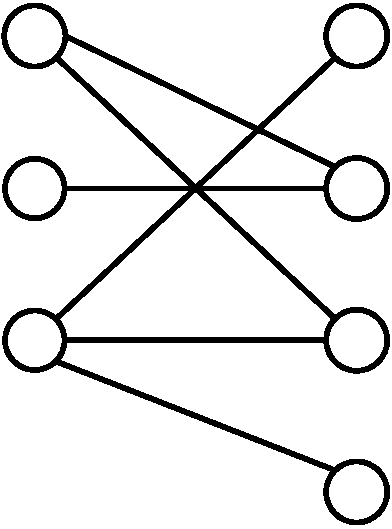
\includegraphics[scale=.25]{../figures/bipartite_graph.pdf}
            \caption{An example of a bipartite graph.}
        \end{figure}
    }

    \only<4>{
        \begin{definition}
            A \textbf{complete bipartite} graph is a bipartite graph where every vertex in one set is 
            adjacent to every vertex in the other set.
        \end{definition}
    }

    \only<5>{
        \begin{definition}
            A \textbf{regular} graph is a graph where each vertex has the same degree. A graph is 
            called K-regular if the degree of each vertex in the graph is K.
        \end{definition}

        \begin{figure}
            \centering
            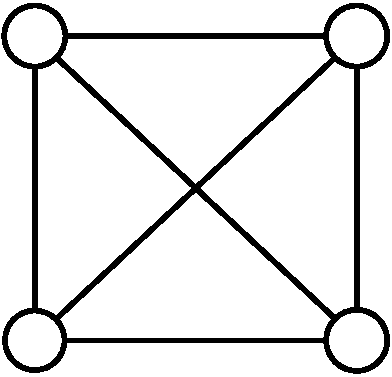
\includegraphics[scale=.25]{../figures/regular_graph.pdf}
            \caption{}
        \end{figure}
    }
}

%%%%%%%%%%%%%%%%%%%%%%%%%%%%%%%%%%%%%%%%%%%%%%%%%%%%%%%%%%%%%%%%%%%%%%%%%%%%%%%%%%%%%%%%%%%%%%%%
%%  Introduction
%%%%%%%%%%%%%%%%%%%%%%%%%%%%%%%%%%%%%%%%%%%%%%%%%%%%%%%%%%%%%%%%%%%%%%%%%%%%%%%%%%%%%%%%%%%%%%%%

\section{Introduction}

\frame{
    A \textbf{party} yields a graph $G$ where people are represented as vertices and two 
    vertices are adjacent if those two people know each other, i.e. are acquaintances.

    \begin{itemize}
        \item<2-> A \textbf{full triangle} is a subset of three people who all know each other. 
        In other words, three adjacent vertices.
        \item<3-> An \textbf{empty triangle} is a subset of three people who are all strangers. 
        In other words, three non-adjacent vertices.
    \end{itemize}
}

%%%%%%%%%%%%%%%%%%%%%%%%%%%%%%%%%%%%%%%%%%%%%%%%%%%%%%%%%%%%%%%%%%%%%%%%%%%%%%%%%%%%%%%%%%%%%%%%
%%  Theorem + Proof
%%%%%%%%%%%%%%%%%%%%%%%%%%%%%%%%%%%%%%%%%%%%%%%%%%%%%%%%%%%%%%%%%%%%%%%%%%%%%%%%%%%%%%%%%%%%%%%%

\section{Theorem One}

\frame{
    \begin{theorem}
        Let $E$ and $F$ be the number of empty and full triangles respectively. 
        Then in every graph with $p$ vertices
        % $$ E + F \geq \binom{p}{3} - \bfloor{ \frac{p}{2} \bfloor{ \bparen{ \frac{p-1}{2} }^2 } } $$
        \begin{equation}
            E + F \geq \binom{p}{3} - \bfloor{ \frac{p}{2} \bfloor{ \bparen{ \frac{p-1}{2} }^2 } } \label{eq:theorem1}
        \end{equation}
        and this lower bound is sharp for each positive integer $p$.
    \end{theorem}
}

\begin{frame}[t]
    \begin{proof}[Proof]\renewcommand{\qedsymbol}{}
        \only<1>{
            Let $P$ be the number of partial triangles in $G$, meaning the number of triangles containing 
            exactly one or two edges. It's clear that
            \begin{equation}
                E + F + P = \binom{p}{3} \label{eq:total_triangles}.
            \end{equation}
        }

        \only<2>{
            Let $d_i$ be the degree of a vertex $v_i$, in other words, the number of people acquainted with 
            the $i^{th}$ person. For each vertex $v_i$, picking one of their $d_i$ acquaintances and one of 
            their $p - 1 - d_i$ nonacquaintances produces a partial triangle. Thus, each $v_i$ produces 
            $d_i(p - 1 - d_i)$ partial triangles.
        }

        \only<3>{
            Furthermore, we note that every partial triangle is counted twice in this manner. To show this
            is true, let vertex $a$, $b$, and $c$ represent $v_i$, one of their acquaintances, and one of 
            their nonacquaintances respectively. Producing a partial triangle from $v_i$ yields two cases.
        }

        \only<4>{
            Case 1: $b$ and $c$ are not acquainted. 
            Then this partial triangle is counted when $v_i$ is $a$ and $v_i$ is $b$.
        }

        \only<5>{
            Case 2: $b$ and $c$ are acquainted. 
            Then this partial triangle is counted when $v_i$ is $a$ and $v_i$ is $c$.
        }

        \only<6>{
            In both cases, the partial triangle is counted twice, which follows for 
            every partial triangle. Consequently,
            \begin{equation}
                P = \frac{1}{2} \sum^{p}_{i=1}{d_i(p - 1 - d_i)} \label{eq:partial_triangles}.
            \end{equation}
        }

        \only<7>{
            Looking back at Equation (\ref{eq:total_triangles}), we can minimize $E + F$ by maximizing $P$.
            To maximize $P$, we must maximize the sum in Equation (\ref{eq:partial_triangles}). We can view 
            each term of the sum as a quadratic function of $d_i$. After finding the derivative of the 
            equation it's clear that we attain our maximum when $d_i = \frac{p - 1}{2}$. 
        }

        \only<8>{
            However, this is a contradiction when $p$ is even since $d_i$ is an integer.
            Thus, if $p$ is odd, we attain the maximum value of $\frac{(p - 1)^2}{4}$ for each term when 
            $d_i = \frac{p - 1}{2}$. If $p$ is even, we attain the maximum possible value of 
            $\frac{p(p - 2)}{4}$ for each term when $d_i = \frac{p}{2}$ or $d_i = \frac{p - 2}{2}$.
        }

        \only<9>{
            In either case, we can express the maximum value as $$ \bfloor{ \bparen{ \frac{p - 1}{2} }^2 }, $$
            and so
            \begin{equation}
                P \leq \frac{1}{2} \sum^{p}_{i=1}{ \bfloor{ \bparen{ \frac{p - 1}{2} }^2 } } 
                    = \frac{p}{2} \bfloor{ \bparen{ \frac{p - 1}{2} }^2 }. \label{eq:partial_max}
            \end{equation}
        }

        \only<10>{
            But since $P$ is an integer, we can strengthen this to read
            \begin{equation}
                P \leq \bfloor{\frac{p}{2} \bfloor{ \bparen{ \frac{p - 1}{2} }^2 }}. \label{eq:p_max}
            \end{equation}
        }

        \only<11>{
            Equations (\ref{eq:total_triangles}) and (\ref{eq:p_max}) now yield our desired bound:
            \begin{equation}
                E + F = \binom{p}{3} - P \geq \binom{p}{3} - \bfloor{\frac{p}{2} \bfloor{ \bparen{ \frac{p - 1}{2} }^2 }}. \label{eq:bound}
            \end{equation}
        }

        \only<12>{
            Next, for each $p$, we must find a graph $G_p$ attaining this bound. But equality in Equation 
            (\ref{eq:theorem1}) is equivalent to equality in Equation (\ref{eq:p_max}) which occurs only 
            when
            \begin{equation}
                P = \frac{1}{2} \sum^{p}_{i=1}{d_i(p - 1 - d_i)} 
                    = \bfloor{\frac{p}{2} \bfloor{ \bparen{ \frac{p - 1}{2} }^2 }}. \label{eq:max_desired}
            \end{equation}
        }

        \only<13>{
            If $p=2n$ for some integer $n$, let $G_p$ be the complete bipartite graph $K_{n,n}$. Now $G_p$ 
            is regular of degree $n$, and we must check that Equation (\ref{eq:max_desired}) is satisfied.
        }

        \only<14>{
            \begin{align*}
                P &= \frac{1}{2} \sum^{p}_{i=1}{d_i(p - 1 - d_i)} & P &= \bfloor{\frac{p}{2} \bfloor{ \bparen{ \frac{p - 1}{2} }^2 }} \notag \\
                  &= \frac{1}{2} \sum^{2n}_{i=1}{n(2n - 1 - n)}   &   &= \bfloor{\frac{2n}{2} \bfloor{ \bparen{ \frac{2n - 1}{2} }^2 }} \notag \\
                  &= \frac{1}{2} \sum^{2n}_{i=1}{n^2 - n}         &   &= \bfloor{ n \bfloor{ \frac{4n^2 - 4n + 1}{4} }} \notag \\
                  &= \frac{1}{2} (2n^3 - 2n^2)                    &   &= \bfloor{ n \bfloor{ n^2 - n + \frac{1}{4} }} \notag \\
                  &= n^3 - n^2                                    &   &= \bfloor{ n(n^2 - n) }  \notag \\
                  &                                               &   &= \bfloor{ n^3 - n^2 } \notag \\
                  &                                               &   &= n^3 - n^2 \notag
            \end{align*}
        }

        \only<15>{
            We can see that Equation (\ref{eq:max_desired}) holds when $p=2n$.
        }

        \only<16>{
            If $p=2n+1$, the construction of $G_p$ is a bit more involved. As depicted for $p=9$ in Figure 
            (\ref{fig:g}), we start with $K_{n,n}$ with its vertices labeled $u_1, u_2,...,u_n$; $v_1, v_2,...,v_n$ 
            and we subdivide edge $u_iv_i$ for $i \leq \frac{n}{2}$. We now obtain $G_p$ by using these 
            $\floor{\frac{n}{2}}$ subdivision points to form a single vertex labeled $w$. We observe that 
            $G_p$ has $2n$ vertices of degree $n$ and one vertex of degree $2\floor{\frac{n}{2}}$. It is 
            routine to check that Equation (\ref{eq:max_desired}) is satisfied.
        }

        \only<18>{
            \begin{align*}
                P &= \frac{1}{2} \sum^{p}_{i=1}{d_i(p - 1 - d_i)}                                                      & P &= \bfloor{\frac{p}{2} \bfloor{ \bparen{ \frac{p - 1}{2} }^2 }} \notag \\
                  &= \frac{1}{2} \sum^{2n+1}_{i=1}{d_i(2n - d_i)}                                                      &   &= \bfloor{\frac{2n+1}{2} \bfloor{ \bparen{ \frac{2n + 1 - 1}{2} }^2 }} \notag \\
                  &= \frac{1}{2} \bparen{\sum^{2n}_{i=1}{n(2n - n)} + 2\floor{\frac{n}{2}}(2n - 2\floor{\frac{n}{2}})} &   &= \bfloor{\frac{2n+1}{2} \bfloor{ n^2 }} \notag \\
                  &= \frac{1}{2} \bparen{\sum^{2n}_{i=1}{n^2} + 2\floor{\frac{n}{2}}(2n - 2\floor{\frac{n}{2}})}       &   &= \bfloor{\bparen{\frac{2n+1}{2}} n^2} \notag \\
                  &= \frac{1}{2} \bparen{2n^3 + 2\floor{\frac{n}{2}}(2n - 2\floor{\frac{n}{2}})}                       &   &= \bfloor{\frac{2n^3+n^2}{2}}  \notag \\
                  &                                                                                                    &   &= \bfloor{ n^3 + \frac{1}{2}n^2 } \notag
            \end{align*}
            At this point, we run into two cases.
        }

        \only<19>{
            Case 1: $n$ is even. Let $n = 2t$ for some integer $t$.

            \begin{align*}
                P &= \frac{1}{2} \bparen{2n^3 + 2\floor{\frac{n}{2}}(2n - 2\floor{\frac{n}{2}})}         & P &= \bfloor{ n^3 + \frac{1}{2}n^2 } \notag \\
                &= \frac{1}{2} \bparen{2(2t)^3 + 2\floor{\frac{2t}{2}}(2(2t) - 2\floor{\frac{2t}{2}})} &   &= \bfloor{ (2t)^3 + \frac{1}{2}(2t)^2 } \notag \\
                &= \frac{1}{2} \bparen{16t^3 + 2t(4t - 2t)}                                            &   &= \bfloor{ 8t^3 + \frac{1}{2}4t^2 } \notag \\
                &= \frac{1}{2} \bparen{16t^3 + 4t^2}                                                   &   &= \bfloor{ 8t^3 + 2t^2 } \notag \\
                &= 8t^3 + 2t^2                                                                         &   &= 8t^3 + 2t^2 \notag
            \end{align*}
        }

        \only<20>{
            Case 2: $n$ is odd. Let $n = 2t + 1$ for some integer $t$.

            \begin{align}
                P &= \frac{1}{2} \bparen{2n^3 + 2\floor{\frac{n}{2}}(2n - 2\floor{\frac{n}{2}})}                                  \notag \\
                  &= \frac{1}{2} \bparen{2(2t + 1)^3 + 2\bfloor{\frac{2t + 1}{2}}(2(2t + 1) - 2\bfloor{\frac{2t + 1}{2}})}        \notag \\
                  &= \frac{1}{2} \bparen{2(8t^3 + 12t^2 + 6t + 1) + 2\floor{t + \frac{1}{2}}(4t + 2 - 2\floor{t + \frac{1}{2}})}  \notag \\
                  &= \frac{1}{2} \bparen{16t^3 + 24t^2 + 12t + 2 + 2t(4t + 2 - 2t)}                                               \notag \\
                  &= \frac{1}{2} \bparen{16t^3 + 28t^2 + 16t + 2}                                                                 \notag \\
                  &= 8t^3 + 14t^2 + 8t + 1                                                                                        \notag \\
                \notag \\
                P &= \bfloor{ n^3 + \frac{1}{2}n^2 }                                                                              \notag \\
                  &= \bfloor{ (2t + 1)^3 + \frac{1}{2}(2t + 1)^2 }                                                                \notag \\
                  &= \bfloor{ 8t^3 + 12t^2 + 6t + 1 + \frac{4t^2 + 4t + 1}{2} }                                                   \notag \\
                  &= \bfloor{ 8t^3 + 12t^2 + 6t + 1 + 2t^2 + 2t + \frac{1}{2} }                                                   \notag \\
                  &= \bfloor{ 8t^3 + 14t^2 + 8t + 1 + \frac{1}{2} }                                                               \notag \\
                  &= 8t^3 + 14t^2 + 8t + 1                                                                                        \notag
            \end{align}
        }

        \only<21>{
            Thus, in both cases, Equation (\ref{eq:max_desired}) holds.
        }

        % \only<>{
            
        % }

        \alt<21>{\qedhere}{\phantom\qedhere}
    \end{proof}

    \begin{figure}
        \centering
        \only<4>{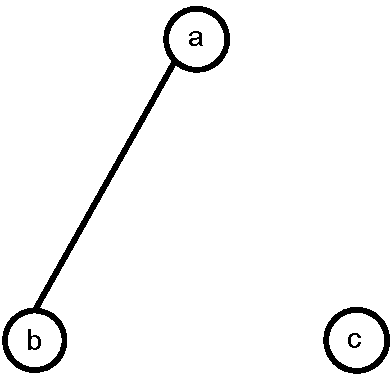
\includegraphics[scale=.25]{../figures/partial_case_1.pdf}}
        \only<5>{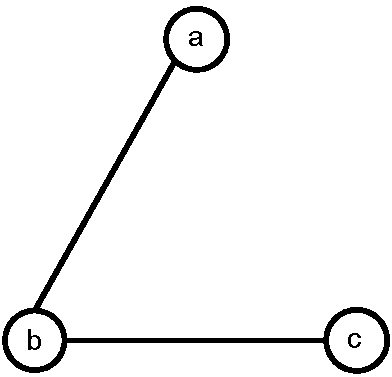
\includegraphics[scale=.25]{../figures/partial_case_2.pdf}}
        \only<17>{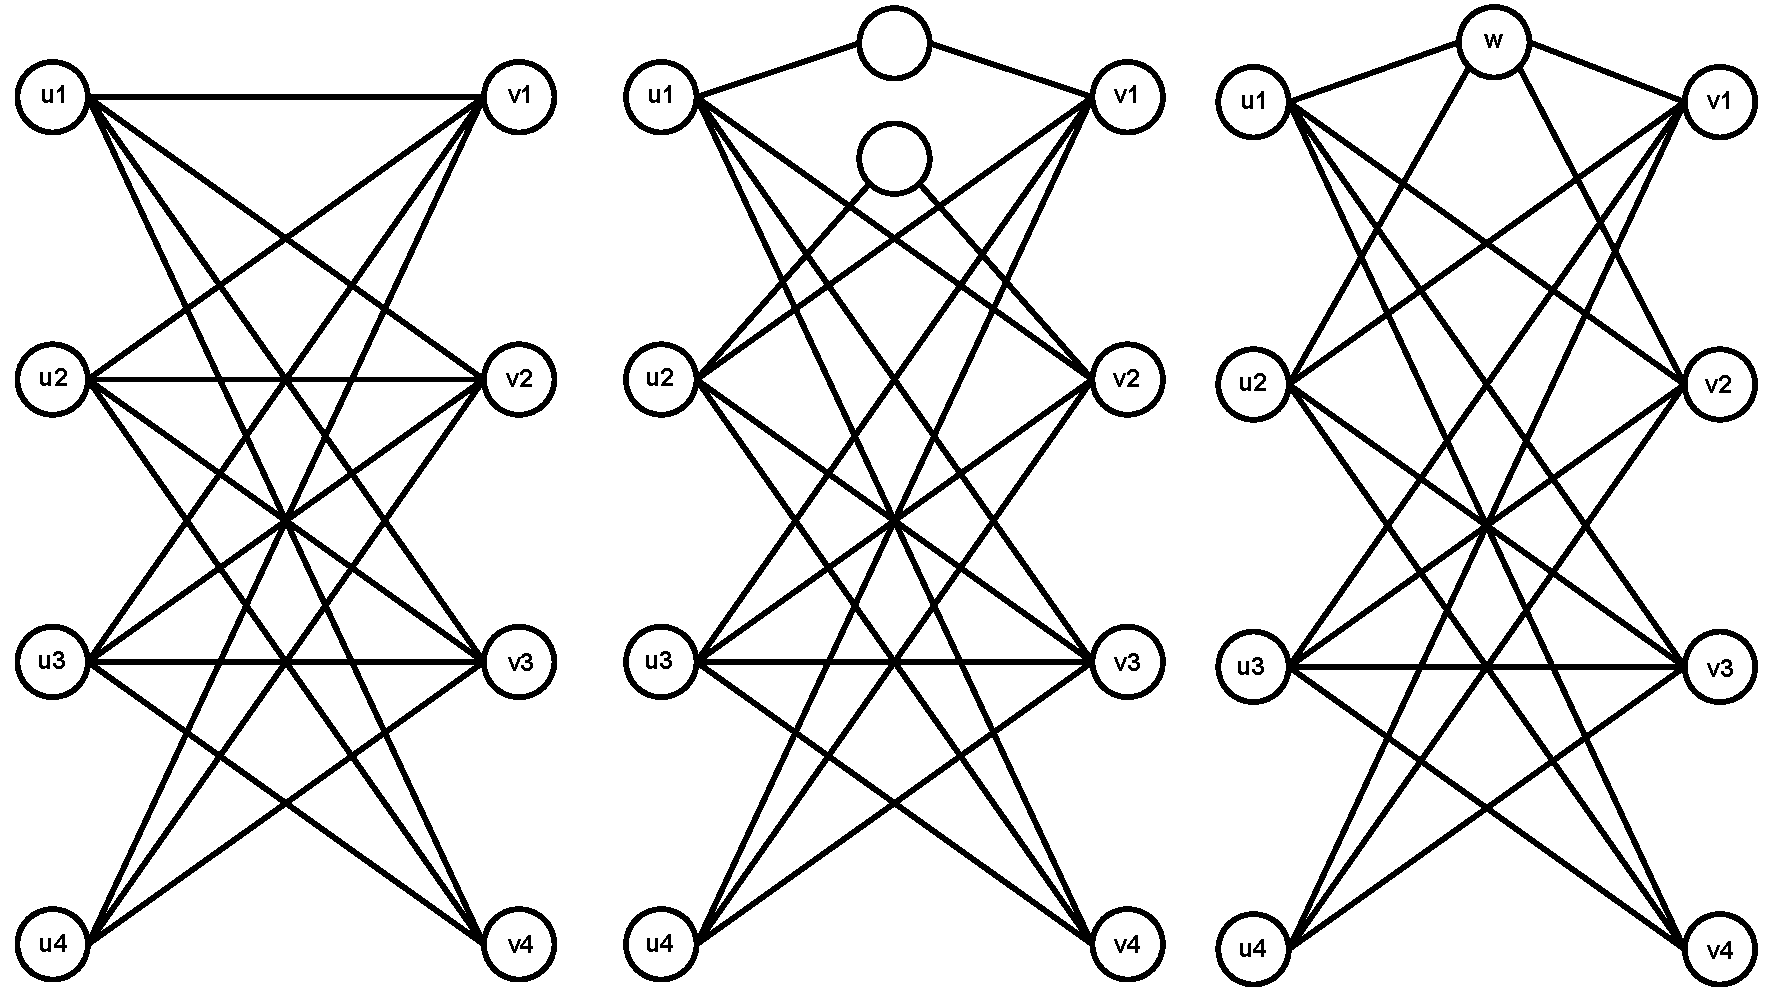
\includegraphics[scale=.25]{../figures/construction_of_g_p.pdf}}
    \end{figure}
\end{frame}

%%%%%%%%%%%%%%%%%%%%%%%%%%%%%%%%%%%%%%%%%%%%%%%%%%%%%%%%%%%%%%%%%%%%%%%%%%%%%%%%%%%%%%%%%%%%%%%%
%%  Theorem + Proof
%%%%%%%%%%%%%%%%%%%%%%%%%%%%%%%%%%%%%%%%%%%%%%%%%%%%%%%%%%%%%%%%%%%%%%%%%%%%%%%%%%%%%%%%%%%%%%%%

\section{Theorem Two}

\frame{
    \begin{theorem}
        In every graph attaining the minimum possible value for E + F,
        \begin{equation}
            F \geq \begin{cases}
                        0 & \text{ if } p = 2n \\
                        n(n - 1) & \text{ if } p = 4n + 1 \text{ or } 4n + 3
                    \end{cases} \label{eq:theorem2}
        \end{equation}
        and this lower bound is sharp for each positive integer $p$.
    \end{theorem}
}

\begin{frame}[t]
    \begin{proof}[Proof]\renewcommand{\qedsymbol}{}
        \only<1>{
            We first observe that this bound is attained by the graphs $G_p$ constructed in the first 
            proof. If $p = 2n$, then $G_p = K_{n, n}$ which obviously has no full triangles. If 
            $p = 4n +1$ or $p = 4n + 3$, we notice that $G_p - w$ is a bigraph, which has no full triangles.
            Thus, every full triangle of $G_p$ has the form $u_i, v_j, w$. But recalling the construction
            of $G_p$, we see that this will be a full triangle if and only if $i \le n$, $j \le n$, and 
            $i \neq j$. Consequently, $G_p$ has $F = n(n - 1)$ full triangles as desired.
        }

        \only<2>{
            It remains to be shown that the bound in Equation (\ref{eq:theorem2}) cannot be violated. If 
            $p$ is even, then this is trivial, since we cannot have a negative number of full triangles. If 
            $p$ is odd and $n = 0$ or $n = 1$, then this is also trivial, since $n(n - 1) = 0$. Therefore,
            we will assume $n \ge 2$.
        }

        \only<3>{
            Case 1: $p = 4n + 1$

            Let $H$ be a graph minimizing $E + F$ with the smallest value of $F$. We will assume $F \le n(n - 1)$
            and show that the bound cannot be violated. A vertex in $H$ lies in an average of $\frac{3F}{4n + 1}$ 
            full triangles, that is, the number of vertices that lie in a full triangle over the total number
            of vertices. Thus, there exists a vertex $v_0$ that lies in $t$ full triangles where
            \begin{equation}
                t \le \frac{3F}{4n + 1} \le \frac{3n(n - 1)}{4n + 1} < n - 1 \label{eq:t_case_1}.
            \end{equation}
        }

        \only<4>{
            Since $t$ and $n$ are integers, we can rewrite this to be $t \le n - 2$. Let $V$ be the vertex set 
            of $H$, let $A$ be the set of vertices adjacent to $v_0$ and let $B$ be the vertices not adjacent to
            $v_0$.
        }

        \only<5>{
            Recall the construction of $G_p$ in the first proof, in order to minimize $E + F$, $H$ must 
            satisfy Equation (\ref{eq:max_desired}) by being a regular graph of degree $2n$. Consequently, 
            there are $2n$ vertices in both $A$ and $B$. Since $v_0$
            lies in $t$ full triangles, there are $t$ edges whose endpoints both lie within $A$.
        }

        \only<6>{
            Now, we know the sum of the degrees of the vertices in $A$ is $4n^2$, we know all $2n$ 
            vertices in $A$ are adjacent to $v_0$, and we know $2t$ vertices in $A$ are adjacent to 
            another vertex within $A$. Thus, there must be $4n^2 - 2n - 2t$ edges joining sets $A$ and $B$. 
        }

        \only<7>{
            Furthermore, there must be $4n^2 - (4n^2 - 2n - 2t) = 2n + 2t$ vertices in $B$ that are adjacent 
            to another vertex in $B$ since no vertex in $B$ is adjacent to $v_0$. Hence, there are 
            $n + t$ edges whose endpoints both lie within $B$.        
        }

        \only<8>{
            Consider an edge $x$ within set $B$. Its two endpoints are incident with $4n - 2$ other edges. 
            Of those edges, at most $n + t - 1$ of them can lie within $B$. Thus, at least 
            $4n - 2 - (n + t - 1) = 3n - t - 1$ edges have an endpoint in $A$. Note that no vertex in 
            $A$ can lie on more than 2 of these edges because that would result in a double edge, and 
            recall that $A$ has $2n$ vertices. 
        }

        \only<9>{
            Therefore, we can conclude that at least 
            $(3n - t - 1) - 2n = n - t - 1$ vertices in $A$ lie on exactly two of these edges. Each of 
            these vertices forms a full triangle containing the edge $x$.
            Thus, each edge within $B$ lies in at least $n - t - 1$ full $ABB$ triangles, and so $H$ should 
            contain at least $(n + t)(n - t - 1)$ full $ABB$ triangles.
        }

        \only<10>{
            Similarly, consider an edge $y$ within set $A$. Its two endpoints are incident with $4n - 2$ other
            edges. Of those edges, we know that two of them have $v_0$ as an endpoint and at most $t - 1$ of 
            them lie within $A$. Thus, at least $4n - 2 - (2 + (t - 1)) = 4n - t - 3$ edges have an endpoint 
            in $B$. Recall that no vertex in $B$ can lie on more than two of these edges and $B$ has $2n$ 
            vertices. 
        }

        \only<11>{
            Consequently, at least $(4n - t - 3) - 2n = 2n - t - 3$ vertices in $B$ lie on 
            exactly two of these edges. Each of these vertices forms a full triangle containing the edge $y$.
            Thus, each edge within $A$ lies in at least $2n - t - 3$ full $AAB$ triangles, and so $H$ should 
            contain at least $t(2n - t - 3)$ full $AAB$ triangles.
        }

        \only<12>{
            Recall that $v_0$ lies on $t$ full triangles. We can add these to the sum of the two bounds that
            we found above to conclude that
            $$ F \ge t + (n + t)(n - t - 1) + t(2n - t - 3) = n^2 - n + 2t(n - t - \frac{3}{2}). $$
            Finally, since $0 \le t \le n - 2$ and $n \ge 2$, we conclude that $F \ge n^2 - n$.
        }

        \only<13>{
            Case 2: $p = 4n + 3$

            As in Case 1, we let $H$ be a graph minimizing $E + F$ with the smallest value of $F$. We 
            will still assume $F \le n(n - 1)$ and again show that the bound cannot be violated. Recall 
            the construction of $G_p$ in the first proof, in order to minimize $E + F$, $H$ must satisfy
            Equation (\ref{eq:max_desired}) by having $4n + 2$ vertices of degree $2n + 1$ and one vertex 
            $w$ of degree $2n$ or $2n + 2$.
        }

        \only<14>{
            Note that a graph with an odd number of vertices cannot be regular 
            with odd degree \cite[Cor. 2.1 (a)]{FH}. We will go ahead and assume $w$ has degree $2n$, for if it were 
            $2n + 2$, we could just remove edges incident with $w$ until we have a graph $H'$ with the desired 
            degrees and $F' \le F$ full triangles.
        }

        \only<15>{
            We continue to repeat the steps in Case 1 by selecting a vertex $v_0$ which does not lie in too
            many full triangles. However, the posibility that $v_0 = w$ is troublesome. Consequently, we select 
            $v_0$ to be a point of degree $2n + 1$ lying in an average of $\frac{3F}{4n + 3}$ 
            full triangles, which is the number of vertices that lie in a full triangle over the total number
            of vertices. Recall that $n \ge 2$, so
            \begin{equation}
                t \le \frac{3F}{4n + 3} \le \frac{3n(n - 1)}{4n + 3} < n - 1 \label{eq:t_case_2}.
            \end{equation}
        }

        \only<16>{
            Since $t$ and $n$ are integers, we can again rewrite this to be $t \le n - 2$. Furthermore, we 
            will define sets $A$ and $B$ the same way that we defined them in Case 1, but now they both contain 
            $2n + 1$ vertices. We will now repeat a similar counting process for the number of full triangles 
            in $H$. However, we must consider two subcases depending on the location of $w$.
        }

        \only<17>{
            Subcase i: $w$ is in $A$

            Then $A$ has $2n$ vertices of degree $2n + 1$ and it has vertex $w$, which has a degree of $2n$. 
            Additionally, $v_0$ lies in $t$ full triangles, so there are $t$ edges whose endpoints both 
            lie within $A$. To add, $B$ has $2n + 1$ vertices of degree $2n + 1$.
        }

        \only<18>{
            Hence, the sum of the degrees of the vertices in $A$ is $4n^2 + 4n$, all $2n + 1$ vertices 
            in $A$ are adjacent to $v_0$, and $2t$ vertices in $A$ are adjacent to another vertex 
            within $A$. Thus, there must be $4n^2 + 4n - (2n + 1) - 2t = 4n^2 + 2n - 2t - 1$ edges 
            joining sets $A$ and $B$.
        }

        \only<19>{
            Then there must be $4n^2 + 4n + 1 - (4n^2 + 2n - 2t - 1) = 2n + 2t + 2$ vertices in $B$ 
            that are adjacent to another vertex in $B$ since no vertex in $B$ is adjacent to $v_0$. 
            Hence, there are $n + t + 1$ edges whose endpoints both lie within $B$.
        }

        \only<20>{
            Consider an edge $x$ within set $B$. Its two endpoints are incident with $4n + 2 - 2$ other edges. 
            Of those edges, at most $n + t$ of them can lie within $B$. Thus, at least 
            $4n - (n + t) = 3n - t$ edges have an endpoint in $A$. Recall that no vertex in $A$ can lie 
            on more than two of these edges and $A$ has $2n + 1$ vertices. 
        }

        \only<21>{
            Therefore, we can conclude that 
            at least $(3n - t) - (2n + 1) = n - t - 1$ vertices in $A$ lie on exactly two of these edges. Each of 
            these vertices forms a full triangle containing the edge $x$.
            Thus, each edge within $B$ lies in at least $n - t - 1$ full $ABB$ triangles, and so $H$ should 
            contain at least $(n + t + 1)(n - t - 1)$ full $ABB$ triangles.
        }

        \only<22>{
            Similarly, consider an edge $y$ within set $A$. Its two endpoints are incident with at least
            $((2n + 1) + 2n) - 2 = 4n - 1$ other edges. Of those edges, we know that two of them have $v_0$ as 
            an endpoint and at most $t - 1$ of them lie within $A$. Thus, at least 
            $4n - 1 - (2 + (t - 1)) = 4n - t - 2$ edges have an endpoint in $B$. Recall that no vertex in $B$ 
            can lie on more than two of these edges and $B$ has $2n + 1$ vertices. 
        }

        \only<23>{
            Consequently, at least 
            $(4n - t - 2) - (2n + 1) = 2n - t - 3$ vertices in $B$ lie on exactly two of these edges. Each of 
            these vertices forms a full triangle containing the edge $y$.
            Thus, each edge within $A$ lies in at least $2n - t - 3$ full $AAB$ triangles, and so $H$ should 
            contain at least $t(2n - t - 3)$ full $AAB$ triangles. 
        }

        \only<24>{
            Recall that $v_0$ lies on $t$ full triangles. We can add these to the sum of the two bounds that
            we found above to conclude that
            $$ F \ge t + (n + t + 1)(n - t - 1) + t(2n - t - 3) = n^2 - 1 + 2t(n - t - 2). $$
            As a result, since $0 \le t \le n - 2$ and $n \ge 2$, we conclude that $F \ge n^2 - n$.
        }

        \only<25>{
            Subcase ii: $w$ is in $B$

            Then $B$ has $2n$ vertices of degree $2n + 1$ and it has vertex $w$, which has a degree of $2n$. 
            It follows that $A$ has $2n + 1$ vertices of degree $2n + 1$. Additionally, $v_0$ lies in $t$ 
            full triangles, so there are $t$ edges whose endpoints both lie within $A$.
        }

        \only<26>{
            Hence, the sum of the degrees of the vertices in $A$ is $4n^2 + 4n + 1$, all $2n + 1$ vertices 
            in $A$ are adjacent to $v_0$, and $2t$ vertices in $A$ are adjacent to another vertex 
            within $A$. Thus, there must be $4n^2 + 4n + 1 - (2n + 1) - 2t = 4n^2 + 2n - 2t$ edges 
            joining sets $A$ and $B$.
        }

        \only<27>{
            Then there must be $4n^2 + 4n - (4n^2 + 2n - 2t) = 2n + 2t$ vertices in $B$ 
            that are adjacent to another vertex in $B$ since no vertex in $B$ is adjacent to $v_0$. 
            Hence, there are $n + t$ edges whose endpoints both lie within $B$.
        }

        \only<28>{
            Consider an edge $x$ within set $B$. Its two endpoints are incident with at least
            $4n + 1 - 2$ other edges. Of those edges, at most $n + t - 1$ of them can lie within $B$. 
            Thus, at least $4n - 1 - (n + t - 1) = 3n - t$ edges have an endpoint in $A$. Recall that 
            no vertex in $A$ can lie on more than two of these edges and $A$ has $2n + 1$ vertices. 
        }

        \only<29>{
            Therefore, we can conclude that at least $(3n - t) - (2n + 1) = n - t - 1$ vertices in $A$ 
            lie on exactly two of these edges. Each of these vertices forms a full triangle containing 
            the edge $x$.
            Thus, each edge within $B$ lies in at least $n - t - 1$ full $ABB$ triangles, and so $H$ should 
            contain at least $(n + t)(n - t - 1)$ full $ABB$ triangles.
        }

        \only<30>{
            Similarly, consider an edge $y$ within set $A$. Its two endpoints are incident with 
            $4n + 2 - 2 = 4n$ other edges. Of those edges, we know that two of them have $v_0$ as 
            an endpoint and at most $t - 1$ of them lie within $A$. Thus, at least 
            $4n - (2 + (t - 1)) = 4n - t - 1$ edges have an endpoint in $B$. Recall that no vertex in $B$ 
            can lie on more than two of these edges and $B$ has $2n + 1$ vertices. 
        }

        \only<31>{
            Consequently, at least 
            $(4n - t - 1) - (2n + 1) = 2n - t - 2$ vertices in $B$ lie on exactly two of these edges. Each of 
            these vertices forms a full triangle containing the edge $y$.
            Thus, each edge within $A$ lies in at least $2n - t - 2$ full $AAB$ triangles, and so $H$ should 
            contain at least $t(2n - t - 2)$ full $AAB$ triangles. 
        }

        \only<32>{
            Recall that $v_0$ lies on $t$ full triangles. We can add these to the sum of the two bounds that
            we found above to conclude that
            $$ F \ge t + (n + t)(n - t - 1) + t(2n - t - 2) = n^2 - n + 2t(n - t - 1). $$
            As a result, since $0 \le t \le n - 2$ and $n \ge 2$, we conclude that $F \ge n^2 - n$.
            In all cases, the bound $F \ge n^2 - n$ cannot be violated when $p$ is odd.
        }

        \alt<32>{\qedhere}{\phantom\qedhere}
    \end{proof}

    \begin{figure}
        \centering
        \only<9>{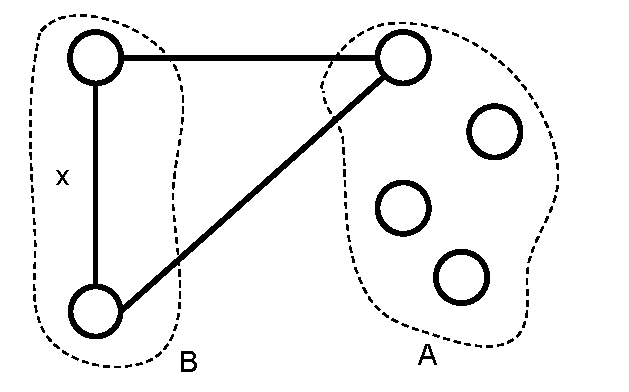
\includegraphics[scale=.25]{../figures/abb_triangle.pdf}}
        \only<11>{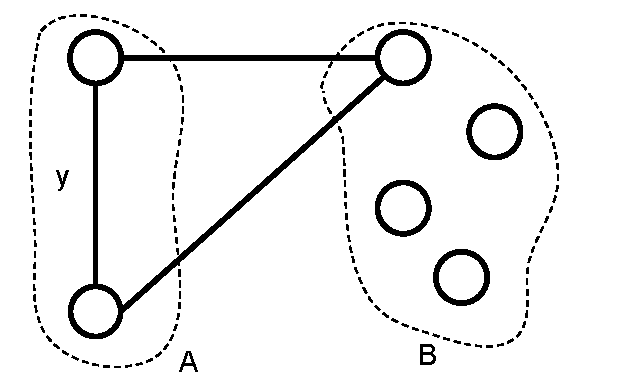
\includegraphics[scale=.25]{../figures/aab_triangle.pdf}}
    \end{figure}
\end{frame}

%%%%%%%%%%%%%%%%%%%%%%%%%%%%%%%%%%%%%%%%%%%%%%%%%%%%%%%%%%%%%%%%%%%%%%%%%%%%%%%%%%%%%%%%%%%%%%%%
%%  Conclusion
%%%%%%%%%%%%%%%%%%%%%%%%%%%%%%%%%%%%%%%%%%%%%%%%%%%%%%%%%%%%%%%%%%%%%%%%%%%%%%%%%%%%%%%%%%%%%%%%

\section{Conclusion}

\begin{frame}
    In conclusion, we observe that when $p$ is even, many graphs attain the bound in Theorem 2. Conversely,
    not many graphs attain that bound when $p$ is odd. In fact, it is even argued that $G_p$ is the unique 
    graph attaining that bound, but the proof is too long to include here.
\end{frame}

%%%%%%%%%%%%%%%%%%%%%%%%%%%%%%%%%%%%%%%%%%%%%%%%%%%%%%%%%%%%%%%%%%%%%%%%%%%%%%%%%%%%%%%%%%%%%%%%
%%  References
%%%%%%%%%%%%%%%%%%%%%%%%%%%%%%%%%%%%%%%%%%%%%%%%%%%%%%%%%%%%%%%%%%%%%%%%%%%%%%%%%%%%%%%%%%%%%%%%

\frame{
    \frametitle{References}
    \begin{enumerate}{
        \scriptsize  
        \item[{[1]}] M. Aigner and G. Ziegler, ``Proofs From THE BOOK," $3^{rd}$ edition, Springer-Verlag, 2004. 203-205
    }\end{enumerate}
}

% \bibitem{AG} A. W. Goodman, \emph{On sets of acquaintances and strangers at any party,} The American Mathematical Monthly {\bf 66} (1959), 778-783.
% \bibitem{FH} F. Harary, ``Graph Theory,'' Addison-Wesley Pub. Co, Reading, Mass., 1969.
% \bibitem{LS} L. Sauv\'e, \emph{On chromatic graphs,} The American Mathematical Monthly {\bf 68} (1961), 107-111.
% \bibitem{AS} A. J. Schwenk, \emph{Acquaintance Graph Party Problem,} The American Mathematical Monthly {\bf 79} (1972), 1113-1117.

\end{document}
